\section{Problem Statement}
\label{sec:problemStatement}

\begin{figure}[t]
\centering
%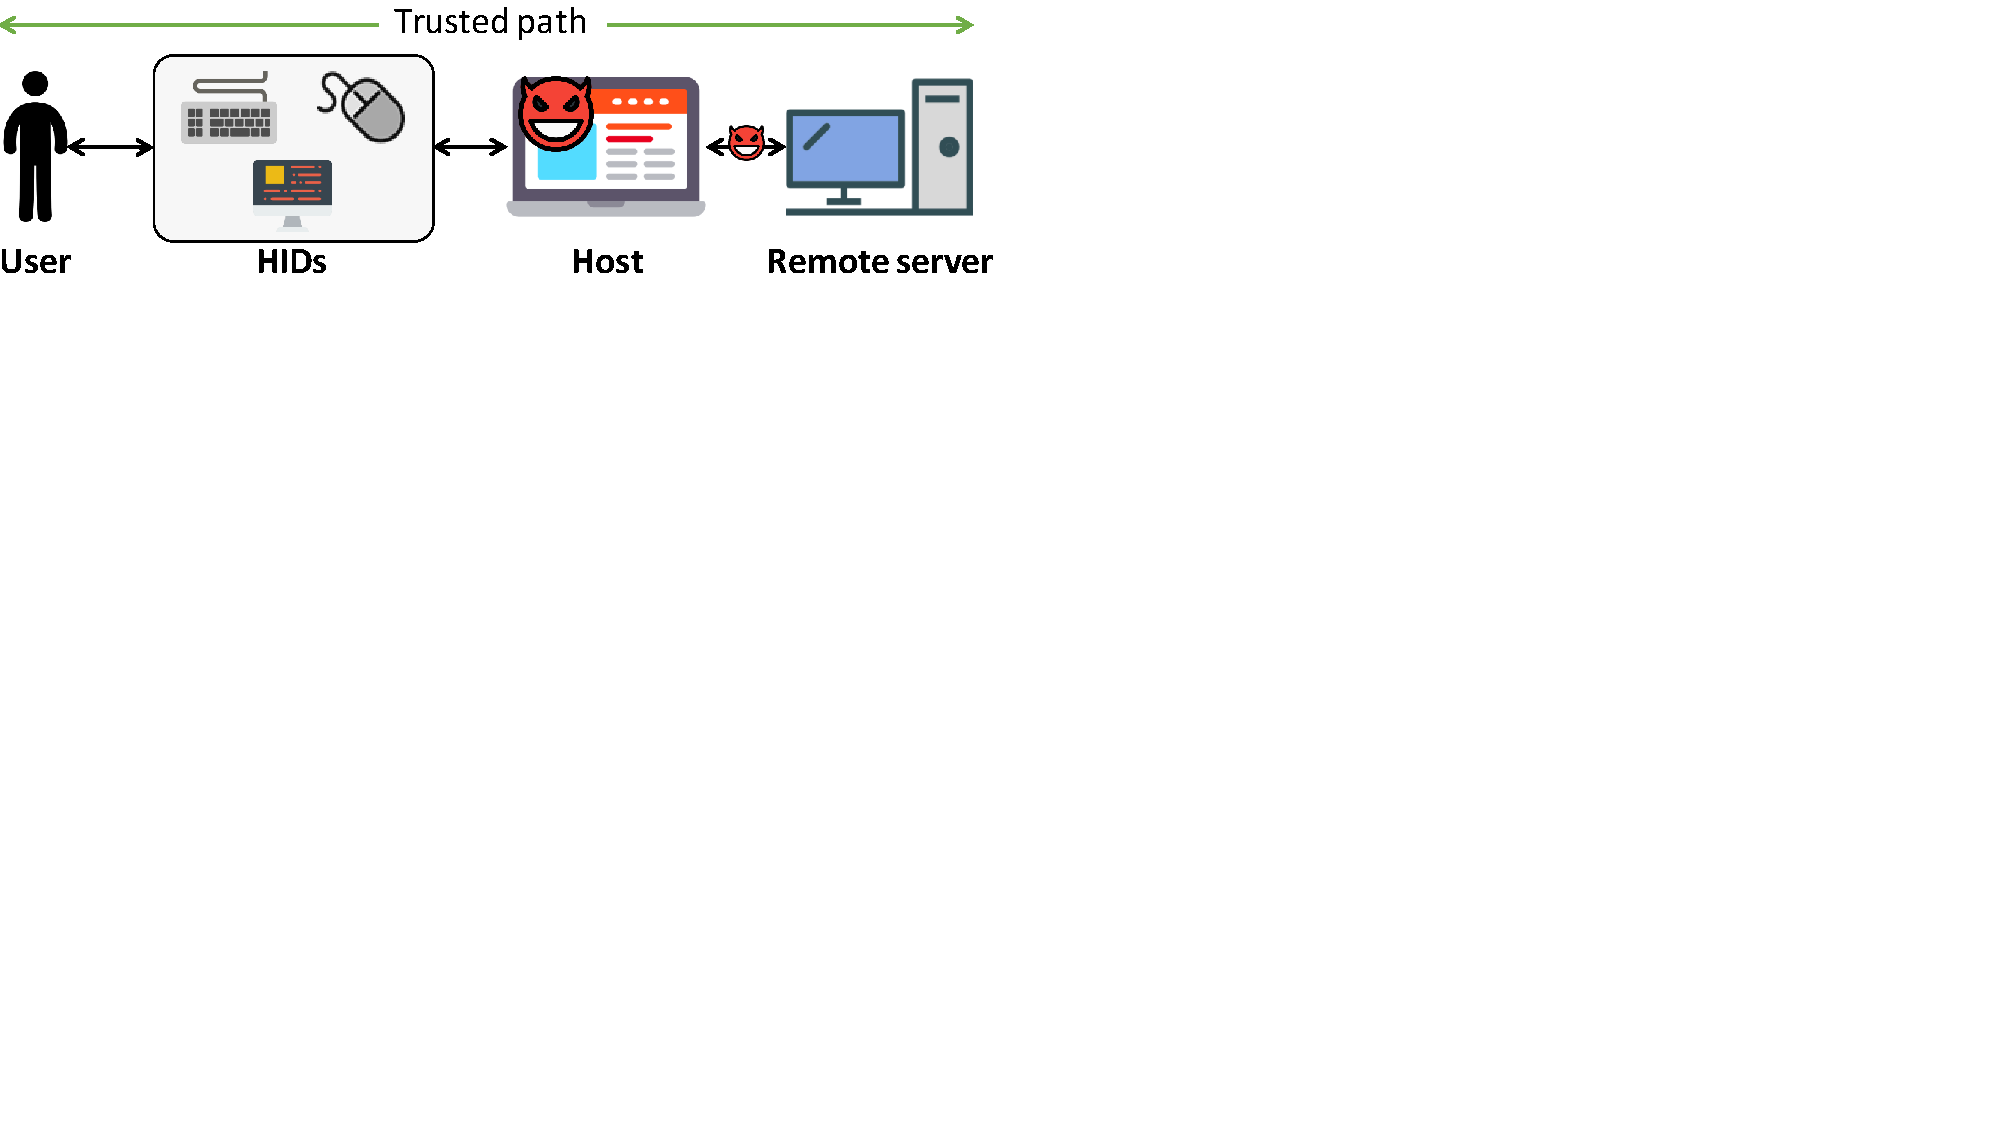
\includegraphics[trim={0 14cm 17cm 0}, clip, width=0.9\linewidth]{systemModel.pdf}
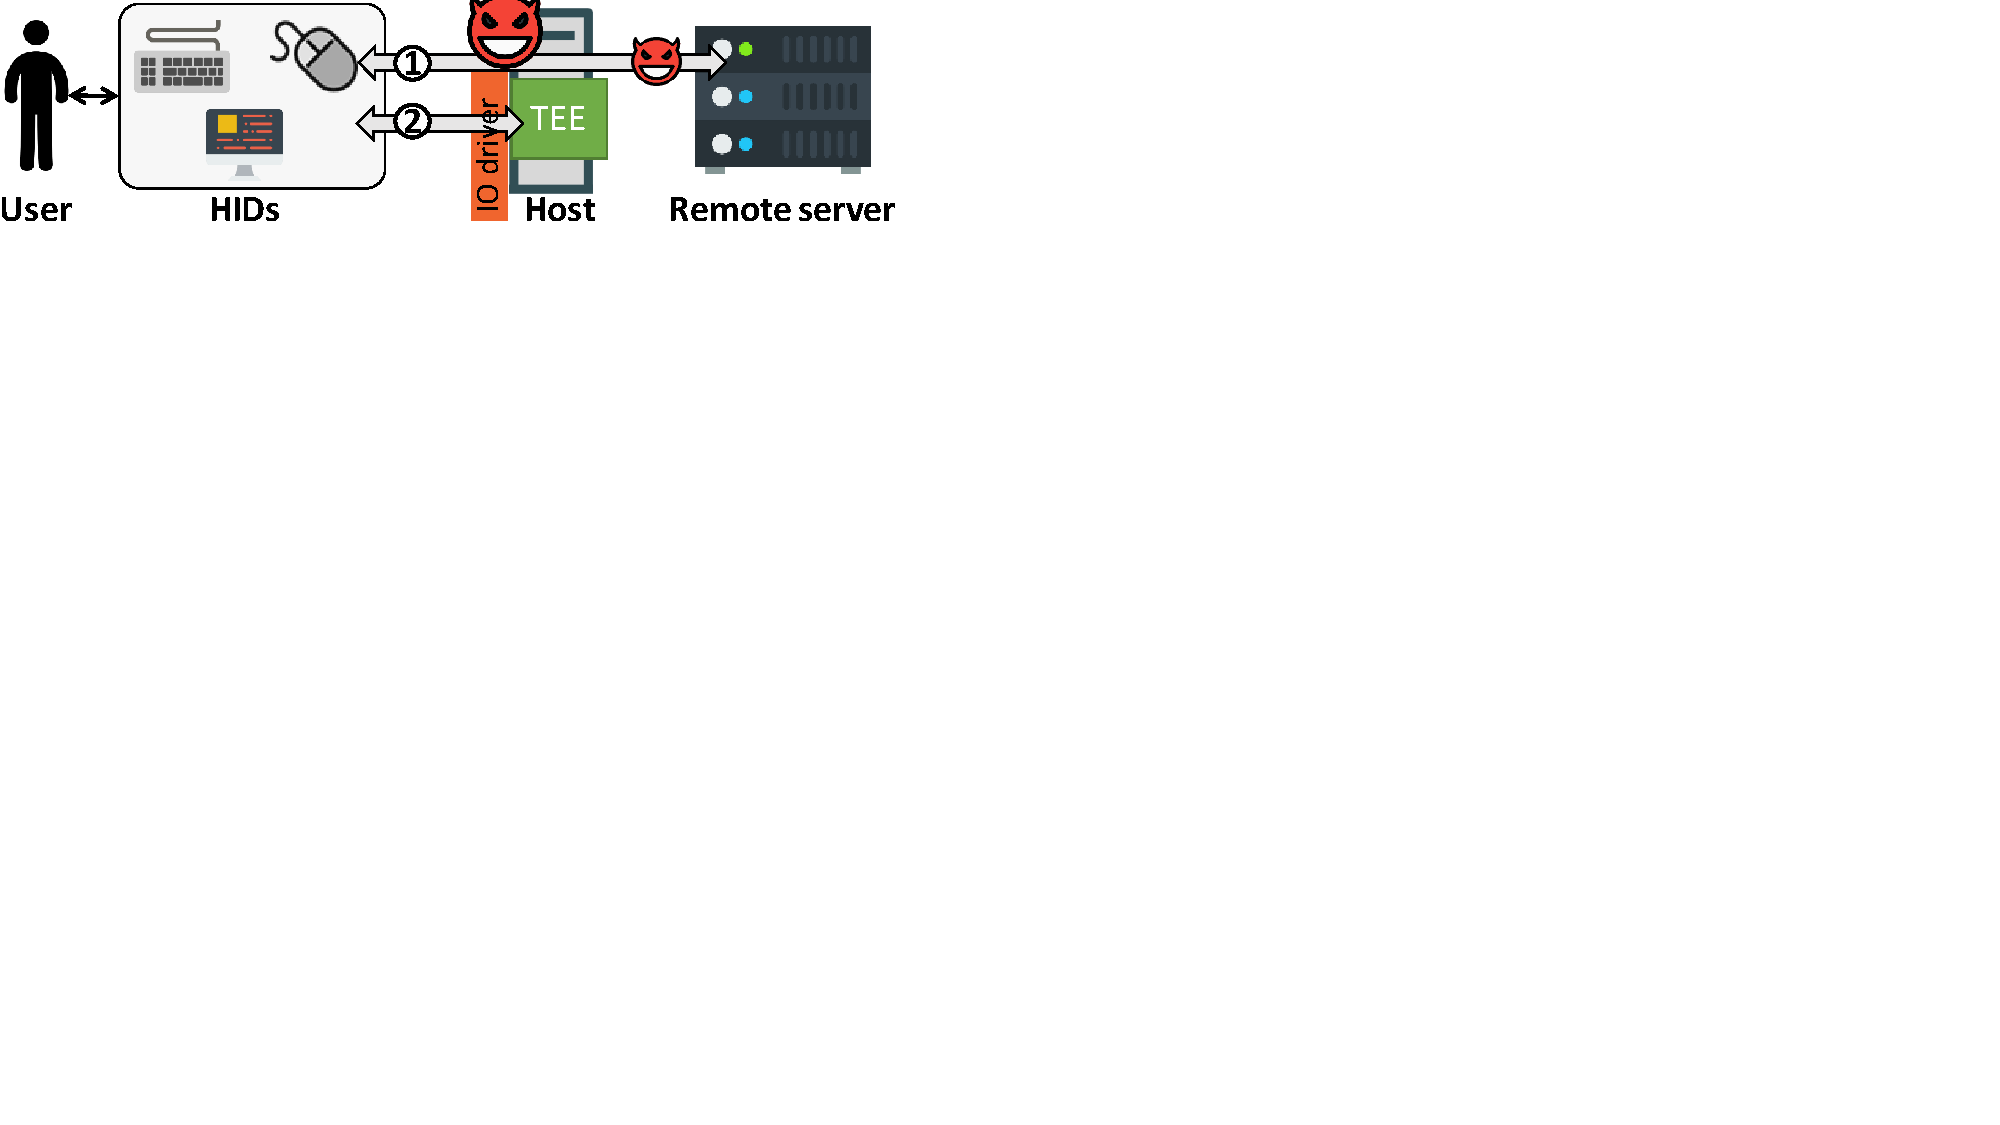
\includegraphics[trim={0 14cm 17cm 0}, clip, width=0.9\linewidth]{systemModel_all.pdf}
\caption{\textbf{Trusted path system model.} The figures shows the system and the attacker model of the trusted path. We generally consider two trusted path scenarios, \one trusted path to a remote server, and \two trusted path to a trusted execution environment (TEE) such as the Intel SGX.}
\label{fig:systemModel}
\centering
\end{figure}


\iffalse
% note: the problem in the current infrastructure: the computer has access to raw data from the server, and the user
A user communicates with a remote server through a host interface which gives %The user typically sends inputs to the server through a keyboard or a mouse and takes responses on a screen. 
the computer access to the plaintext data that goes from the user to the server and vice-versa. Thus, an adversary that compromises the user's host can easily steal or modify the information going on any directions to alter user intentions, i.e., it performs arbitrary actions on behalf of the user. Such an adversary is very powerful and difficult to be detected or prevented by a remote server. The consequences of such attacks are critical when targeting high-importance applications. The attacker can read all sensitive communication of the user, redirect user's payments to a malicious account, or even threaten individuals lives by misconfiguring a medical device.

% note: full compromise is possible in many ways, so we need trusted channels
The complexity of nowadays computer systems does not restrict such attackers, but on the contrary it opens up new possibilities. The adversary can jeopardize user inputs or outputs by attacking the user's computer directly, e.g., Man-in-The-Browser (MiTB) attacks, keyloggers, or malwares that can escalate their privileges to gain root access on the system. Furthermore, many sensitive applications offer their services via a native application or a website that usually imports third-party libraries. An adversary can craft a malicious piece of code and add it on a popular open source library to attack user inputs on specific applications, known as software supply chain attacks. This kind of attack is already seen on the past for websites managing cryptocurrencies wallets~\cite{softSupplyChainAttack, jsSupplyChainAttack}. Therefore, the necessity of a trusted channel between the remote server and the user is critical in any sensitive application.

%To mitigate these attacks, in some specific applications, e.g., online payments, the remote server asks the user to confirm her action on a second device (phone or special hardware). However, this defense mechanism is possible on very limited use-cases and it only prevents the adversary from altering the user action, but the sensitive information still leaks. 

%note: inspiration and what do we need
The existing systems do not provide any interface to the remote server to learn if the user's machine is compromised or not. Trusted execution environments (TEEs) such as Intel SGX bring trust into the processor, effectively eliminating the need to trust more significant code base (motherboard, memory modules, OS and other applications). However, the problem of isolating user's input and output remains as the operating system handles the IO drivers and data. Therefore, service providers typically operate with the assumption that the data they receive are genuinely generated by honest users and not altered by a compromised computer. On a few use cases, e.g., online payments, the service providers ask for user confirmation on a second device (phone or special hardware) to prevent such attacks. However, this solution is limited to few applications and it only gives integrity (the attacker still learns all inputs) for the user inputs. Our goal is to design a solution that does not require significant changes into the current infrastructure and provides the following features: (i) input integrity and privacy, (ii) output integrity and privacy, (iii) sandboxed mouse pointer movements, and (iv) low-TCB.

%Security properties such as integrity and privacy protect user's data from an adversary who wants to either make arbitrary changes to the data or see the sensitive data. Trusted execution environments (TEEs) such as Intel SGX supports isolation execution environments that protect the sensitive application from a malicious application. Privacy of the application data is achieved through memory encryption that hides the sensitive user/application data from the operating system. Remote attestation ensures that the target platform runs the proper version of an enclave. There also exists other TEEs that provides a similar set of features. Technologies such as Intel SGX bring trust into the processor, effectively eliminating the need to trust more significant code base (motherboard, memory modules, OS and other applications). But the problem of isolating user's input and output remains as the operating system handles the IO drivers and data. There exists some solution of building a trusted path between the user and the protected applications (enclaves in the SGX terminology), none of the existing methods providers a robust and generic solution that requires very few changes into the current and legacy system.

%In this paper, we tackle the problem of securing sensitive user IO data from arbitrary IO devices. We assume that the attacker compromises host systems that include the hardware, the operating systems, and all the installed applications. Such an attacker model allows it not only to steal the sensitive information from the user but also alter them. Additionally, as the attacker is in full control of the host system, he can alter the UI elements on the screen, change the location of the pointer, modify the speed and the acceleration of the pointer, etc. Such a capability of the attacker makes the problem of protecting the integrity of the mouse pointer a challenging one. Even though the problem of preserving the integrity/privacy of the keyboard input is addressed in the recent literature, integrity/privacy for mouse pointer is still an unsolved problem. Furthermore, the user is completely unprotected, she cannot verify that her inputs are transferred to the server securely, or even have the guarantee that she is communicating with the legitimate server. 

%In other words, in this paper, we focus on a new way to build systems that bring a user's trust into IO devices and data - keeping in mind that the solution works by almost no or little changes to the existing systems. Additionally, we also assume that the user's platform may nor support any TEEs. Such assumption reduces the trusted code base to bare minimal and making the problem of protecting user IO data under strong adversary model a challenging task.      
\fi

In this section, we motivate our work, explain the security properties, describe exiting literature lacks proper solution and explain the goals of our work.


\begin{table*}[t]
\scriptsize
\centering
%\bgroup
%\def\arraystretch{1.2}
\resizebox{\textwidth}{!}{
  \begin{tabular}{l | l | c  c  c  c | c  c  c  c} 
   \multirow{3}{*}{Category}
   & &\multicolumn{4}{c|}{Trust Assumption} & \multicolumn{4}{c}{IO Protection}\\  \cline{3-10}
   & &\multicolumn{2}{c|}{Hardware} & \multicolumn{2}{c|}{Software} & \multicolumn{3}{c|}{Input} & \multicolumn{1}{c}{Output} \\  \cline{3-10}
   %\rowcolor{Gray}
   \cellcolor{white} & & Requires TEE & \multicolumn{1}{c|}{External trusted HW} & Isolated API/Drivers & Hypervisor/OS & Keyboard & Pointer & \multicolumn{1}{c|}{Touch} & Display \\
   \hline
    &Browser-based~\cite{ye2005trusted}			 & \no 		& \no  	& \yes 		& \yes 	& \no 			& \no 	& \no 		& \yesNope\\
    \rowcolor{Gray}
   	\cellcolor{white} & InContext~\cite{Overshadow} 				 & \no 		& \no 	& \no 	  	& \yes 	& \no 			& \yes 	& \no 		& \no\\
    & Overshadow~\cite{Overshadow} 				 & \no 		& \no 	& \no 	  	& \yes 	& \no 			& \no 	& \no 		& \no\\
    \rowcolor{Gray}
    \cellcolor{white}&Virtual ghost~\cite{criswell2014virtual} 	 & \no 		& \no 	& \no 		& \yes 	& \no 			& \no 	& \no 		& \no\\
    &TrustVisor~\cite{mccune2010trustvisor} 		 & \no 		& \no 	& \no 		& \yes 	& \no 			& \no 	& \no 		& \no\\
    \rowcolor{Gray}
    \cellcolor{white}&Inktag~\cite{hofmann2013inktag} 			 & \no 		& \no 	& \no 		& \yes 	& \no			 & \no 	& \no 		& \no\\
    &Splitting interfaces~\cite{ta2006splitting}  & \no 		& \no 	& \no 		& \yes 	& \yes 			& \no 	& \no 		& \yes\\
    \rowcolor{Gray}
    \cellcolor{white}&$SP^3$~\cite{yang2008using} 				 & \no 		& \no 	& \no 		& \yes 	& \yes 			& \no 	& \no 		& \no\\
    &SGX IO~\cite{weiser2017sgxio}  				 & \yes 	& \no 	& \yes 	& \yes	& \yes 			& \no 	& \no 		& \no\\
    \rowcolor{Gray}
    \cellcolor{white}\parbox[t]{1mm}{\multirow{-11}{*}{\rotatebox[origin=c]{90}{\textbf{Hypervisor/OS-based}}}}  \ldelim\{{-10}{0mm}[] & SchrodinText~\cite{sani2017schrodintext}	 & \yes 	& \no  & \no 	& \yes 	& \no 			& \no 	& \no 		& \yes\\
    &BASTION-SGX~\cite{BASTION-SGX}			     & \yes 	& \no  	& \no 		& \no 	& \yes 			& \no 	& \no 		& \no\\
    \rowcolor{Gray}
    \cellcolor{white}&Slice~\cite{azab2011sice}				     & \yesNope & \no  	& \no 		& \no 	& \no 			& \no 	& \no 		& \no\\
    &TrustOTP~\cite{sun2015trustotp}			     & \yes 	& \no  	& \no 		& \no 	& \yes		 	& \no 	& \no 		& \yesNope\\
    \rowcolor{Gray}
    \cellcolor{white}&VeriUI~\cite{liu2014veriui}				     & \yes 	& \no  & \yes 		& \no 	& \yesNope 		& \no 	& \no 		& \yesNope\\
	&AdAttester~\cite{li2015adattester}			 & \yes 	& \no  & \yes 		& \no 	& \no 			& \no & \yesNope 	& \yesNope\\
	\rowcolor{Gray}
	\cellcolor{white}&TruZ-Droid~\cite{ying2018truz}			     & \yes 	& \no  & \yes 		& \no 	& \yes 			& \no 	& \no 		& \yesNope\\
	&TrustUI~\cite{li2014building}			     & \yes 	& \no  & \yesNope 	& \no 	& \no 			& \no 	& \yesNope 		& \yesNope\\
	\rowcolor{Gray}
	\cellcolor{white}&VButton~\cite{li2018vbutton}			     & \yes 	& \no  & \yes 	& \no 	& \yesNope 			& \no 	& \yes 		& \yes\\
    &CARMA~\cite{vasudevan2012carma}			     & \yes 	& \yes 	& \no 		& \no 	& \no 			& \no 	& \no 		& \no\\
    \rowcolor{Gray}
    \cellcolor{white}&\textsc{ProximiTee}~\cite{dhar2018proximitee}&\yes 		& \yes  & \yesNope 	& \no 	& \yes 			& \no 	& \no 		& \no\\
     \cellcolor{white}\parbox[t]{3mm}{\multirow{-13}{*}{\rotatebox[origin=c]{90}{\textbf{TEE-based}}}}  \ldelim\{{-13}{0mm}[] & Fidelius~\cite{Fidelius}			   	     & \yes 	& \yes  & \yes 		& \no 	& \yes 			& \no 	& \no 		& \yesNope\\
    \rowcolor{Gray}
    \cellcolor{white}&FPGA-based~\cite{brandon2017trusted}		 & \no 		& \yes  & \no 		& \no 	& \yes 			& \no 	& \no 		& \yes\\
    &IntegriKey~\cite{IntegriKey}				 & \no 		& \yes  & \yesNope 	& \no 	& \yesNope 		& \no 	& \no 		& \no\\ 
    \rowcolor{Gray}
    \cellcolor{white} \cellcolor{white}\parbox[t]{5mm}{\multirow{-6}{*}{\rotatebox[origin=c]{90}{\textbf{External HW}}}}  \ldelim\{{-6}{0mm}[] &Terra~\cite{garfinkel2003terra}			     & \no 		& \yes  & \yesNope 	& \no 	& \no 			& \no 	& \no 		& \no\\   
    
	\rowcolor{HGray}
	\cellcolor{white}&\textbf{\name}	    			& \no 		& \yes  & \no 		& \no 	& \yes 			& \yes 	& \yes 		& \yes\\
    \hline
    \multicolumn{10}{c}{\small\yes~requires/supports \hspace{1cm} \no~not requires/supports \hspace{1cm} \yesNope ~partially requires/supports}  
  \end{tabular}
  }
  \caption{\textbf{Summarization of existing trusted path solutions} by their trust assumptions and security features. Note that a lower trust assumption and a high number of security features are desired from a generic trusted path solution. \red{To be moved in Appendix}}
  \label{tab:relatedWorks}
\end{table*}



\iffalse
\tikzstyle{line}=[draw] 
\begin{figure}[t]
\small
    \centering
\begin{tikzpicture}[level distance=10mm, 
  sibling distance=10mm,
  nodex/.style={fill=green!20,rectangle,rounded corners,draw},
  node1/.style={fill=black!5,rectangle,rounded corners,draw},
  node2/.style={fill=white,rectangle},
  arrow/.style={edge from parent/.style={draw,-latex}}
]

\node[node1] {Trusted path}
child[grow=right] {
child[arrow] {node[node1](h){Hypervisor}} child[arrow] {node[node1](htee){Hypervisor + TEE}} child[arrow] {node[node1](tee){TEE}} child[arrow] {node[node1, xshift=15pt](br){Browser-based}} child[arrow] {node[node1](teehw){TEE + External HW}} child[arrow] {node[nodex](hw){External HW}}};

\node[node2, right=5pt of hw] {\textbf{\name}};
\node[node2, right=5pt of br] {InContext~\cite{blake1998authenticated}};
\node[node2, right=5pt of htee] {SGX IO~\cite{weiser2017sgxio}};
\node[node2, right=5pt of tee] {BASTION-SGX~\cite{BASTION-SGX}	};
\node[node2, right=5pt of teehw] {Fidelius~\cite{Fidelius}};
\node[node2, right=5pt of h] {Overshadow~\cite{Overshadow}};
\end{tikzpicture}
    \caption{\textbf{Summarization of existing trusted path solutions} by their trust assumptions. Detailed description of the related works is discussed in Table~\ref{tab:relatedWorks}.}
    \label{fig:relatedWorksTree}
\end{figure}
\fi


\begin{figure}[t]
\footnotesize
    \centering
    \begin{tikzpicture}[
solved/.style={rectangle,draw,fill=purple!40, rounded corners, align=center},
not/.style={rectangle, draw,fill=orange!60, rounded corners, align=center},
neutral/.style={rectangle, draw, rounded corners, align=center, fill=black!5}
]]
    \node[neutral](root) {Trusted path}
    child { node[neutral, yshift=12pt] (hw) {External\\ HW}}
    child { node[neutral, yshift=8pt, xshift=10pt] (tc) {Transaction\\ confirmation\\ Device}}  
    child { node[neutral, yshift=12pt, xshift=20pt] (tee) {TEE}
      child { node[neutral, yshift=0pt, xshift=-5pt] (teehv) {Hypervisor+\\TEE}}
      child { node[neutral, yshift=0pt, xshift=2pt] (teehw) {TEE + \\ External HW} } }
      child { node[neutral, yshift=8pt, xshift=15pt] (br) {Browser\\ Based}}   
     child { node[neutral, yshift=12pt, xshift=20pt] (hv) {Hypervisor}}  ;
    
      

    \node[below=0cm of hw] {\textbf{\name}};
    \node[below=0cm of tc] {Uni-dir~\cite{filyanov2011uni}};
    \node[below=0cm of hv] {Overshadow~\cite{Overshadow}};
    \node[below=0cm of teehv] {SGXIO~\cite{weiser2017sgxio}};
    \node[below=0cm of teehw] {Fidelius~\cite{Fidelius}};
     \node[below=0cm of br] {InContext~\cite{blake1998authenticated}};

    
    \end{tikzpicture}
    
   \caption{\textbf{Summarization of existing trusted path solutions} by their trust assumptions. Detailed description of the related works is discussed in Table~\ref{tab:relatedWorks}.}
     \label{fig:relatedWorksTree}
\end{figure}


\subsection{Motivation: IO for Remote Data and Safety-critical System}


A user communicates with a remote server through a computer interface, we call it as the host system, which gives the host access to the plaintext data that goes from the user to the server and vice-versa. Thus, a compromised host can always steal or modify the information going on both directions. An adversary that compromises the user's host can alter user intentions, i.e., it can perform arbitrary actions on behalf of the user. Such an adversary is very powerful and difficult to be detected or prevented by a remote server. The consequences of such attacks might be very serious when high-importance applications are targeted. The attacker can read all sensitive communication of the user, redirect user's payments to a malicious account, or even threaten individuals lives by misconfiguring a medical device.  For example, passing the wrong input to a remote safety-critical system such as a medical device, power plant, etc. can be disastrous.


\iffalse
The complexity of nowadays computer systems does not restrict such attackers, but on the contrary it opens up new possibilities. The adversary can jeopardize user inputs or outputs by attacking the user's computer directly, e.g., Man-in-The-Browser (MiTB) attacks, keyloggers, or malwares that can escalate their privileges to gain root access on the system. Furthermore, many sensitive applications offer their services via a native application or a website that usually imports third-party libraries. An adversary can craft a malicious piece of code and add it on a popular open source library to attack user inputs on specific applications, known as software supply chain attacks. This kind of attack is already seen on the past for websites managing cryptocurrencies wallets~\cite{softSupplyChainAttack, jsSupplyChainAttack}. Therefore, the necessity of a trusted channel between the remote server and the user is critical in any sensitive application.
\fi
%To mitigate these attacks, in some specific applications, e.g., online payments, the remote server asks the user to confirm her action on a second device (phone or special hardware). However, this defense mechanism is possible on very limited use-cases and it only prevents the adversary from altering the user action, but the sensitive information still leaks. 

%note: inspiration and what do we need
%The existing systems do not provide any interface to the remote server to learn if the user's machine is compromised or not. 
Trusted execution environments (TEEs) such as Intel SGX bring trust into the processor, effectively eliminating the need to trust more significant code base (motherboard, memory modules, OS and other applications). However, the problem of isolating user's input and output remains as the operating system handles the IO drivers and data. Therefore, service providers typically operate with the assumption that the data they receive are genuinely generated by honest users and not altered by a compromised computer. On a few use cases, e.g., online payments, the service providers ask for user confirmation on a second device (phone or special hardware) to detect such attacks. However, this solution is limited to few applications and it only provides integrity (the attacker still learns all details) for the user inputs. 
%Our goal is to design a solution that does not require significant changes into the current infrastructure and provides the following features: (i) input integrity and privacy, (ii) output integrity and privacy, (iii) sandboxed activity, and (iv) low-TCB.

\subsection{Fine-grained Security Properties}

As we discussed in the previous section, \emph{Trusted paths} provide the security properties (privacy and integrity) to the IO data between the users and the end systems. In principle trusted paths solve the general security problem of the IO data. But practically establishing a trusted path in general IO devices is a nontrivial problem specifically if one considers the plethora of complex UI objects and input methods.

We list the fine-grained security properties that we want to provide in our proposed solution. We now discuss these security properties and corresponds them with the motivating example.

\begin{mylist}
  \item \textbf{Input integrity and privacy.} These properties define that any input that is coming from the user input devices are fully protected in two ways: i) the input issued by the user reaches to the remote end-point as it was meant to be - \emph{integrity}, and ii) in specific application scenarios, the attacker-controlled host is entirely oblivious about the input from the user - \emph{privacy}. The input may come from arbitrary input devices, such as keyboard, mouse, touch etc. We consider any sort of input action by the user that may include moving the mouse or using the keyboard navigation keys to select a specific item in a list.
  
  %We can further fine grain the user input to the granularity of user-issued \emph{commands} and \emph{mouse movements}. Both of which are generated by the input devices from the user. User-issued commands are the specific actions that are executed by the user. Commands are transmitted to the remote end-system, e.g., filling a text-box with a parameter and clicking the \emph{submit} button issues a \texttt{HTTP} request to the remote server. The mouse movements are actions that are given to the host system which are not directly transmitted to the remote end-system but causes user-issued commands, e.g., mouse movement from one point to a button that user intends to click. In a word, user-issued commands changes the state on the remote server while the mouse movements does not change the state on the remote server.  
  
  \item \textbf{Output integrity and privacy.} Similar to the input integrity, output integrity ensures that information that is sent by the remote endpoint is presented to the user as it was meant to be. One example of output integrity is the integrity of the UI elements. Such property ensures that the host system renders the UI elements faithfully as they were sent by the remote system. 
  %We further fine-grain output integrity and privacy by dividing it into two parts: \emph{data} and \emph{UI}. Data denotes the information that is passed from a remote entity to the host and UI denotes to the user interface structure that is presented to the user.

  As proven on the Section \ref{inputTheoryAritra}, ensuring output integrity is essential for providing input integrity against advanced attackers that trick the user to send non-legitimate data to the server. For example, the user wants to send a number \texttt{10} to the server, but the malicious host shows on screen \texttt{100} and fools the user into believing he mistyped a \texttt{0}. The user deletes one \texttt{0} and sees \texttt{10} on the screen---as he intended initially---and submits the data, however, on the server arrives just \texttt{1}. 
  
  Providing output integrity is a challenging task even on systems that have a trusted component that overlays parts of the HDMI frames generated by the untrusted host. Previous works~\cite{huang2012clickjacking} show that when  a trusted component and an untrusted one share a screen, the attacker can still manipulate the user to commit unintentional actions to the trusted UI if the system is not designed properly. In our solution we want to guarantee that the user is aware of the UI elements (trusted or untrusted) that she interacts with, therefore preventing related attacks.
  \end{mylist}



\iffalse
\myparagraph{Advantages}

\begin{enumerate}
  \item The \device does not need to know the formatting/template of the page. As the \device only looks to the current mouse position, the structure of the page is somewhat irrelevant (?).
\end{enumerate}
\fi

\iffalse
\begin{table}[t]
\small
\centering
  \begin{tabular}{ l | c | c }
    \hline
     & TEE & no TEE \\ \hline
    \multirow{6}{*}{Hypervisor-based} & \multirow{6}{*}{SGX IO~\cite{weiser2017sgxio}} & Overshadow~\cite{Overshadow} \\ 
    & & Virtual ghost~\cite{criswell2014virtual}\\ 
    & & Inktag~\cite{hofmann2013inktag}\\ 
    & & TrustVisor~\cite{mccune2010trustvisor} \\ 
    & & Splitting interfaces~\cite{ta2006splitting}\\ 
    & & $SP^3$~\cite{yang2008using}\\ \hline
   Isolated execution & BASTION-SGX~\cite{BASTION-SGX} & Slice~\cite{azab2011sice}\\ 
   of APIs/Drivers & TrustOTP~\cite{sun2015trustotp} & CARMA~\cite{vasudevan2012carma} \\ \hline
   External trusted  &  \multirow{2}{*}{Fidelius~\cite{Fidelius}} & IntegriKey~\cite{IntegriKey} \\
   hardware based &  & FPGA-based~\cite{brandon2017trusted} \\
    %&  & \textcolor{blue}{Our Solution (I + O + Activity)} \\
    \hline
    Handles both & \multirow{2}{*}{\textcolor{red}{None}} & \multirow{2}{*}{\textcolor{blue}{Our Solution}} \\
    keyboard + mouse &  & \\
    \hline
  \end{tabular}
  \caption{Summarization of existing trusted path solutions. Note that in the table, switching systems from left to right or top to bottom, reduces the trust assumption. For example, TEE based solutions, such as SGX-based trusted path solution requires trust on the physical processor packages, SGX APIs, quoting and launch enclaves and Intel attestation service.}
\end{table}
\fi


\subsection{Existing Solutions and their drawbacks}

There exists several works that try to solve the problem of trusted paths for IO devices in the presence of a compromised host. But all of these solutions targeted for different problem settings and models. Figure~\ref{fig:relatedWorksTree} provides a board classification of the related works and illustrates where our proposed work stands with respect to them. Detailed description of the related research is also described in Table~\ref{tab:relatedWorks}.

\subsubsection{Trusted Execution Environments} TEEs are other ways to implement a trusted path between the IO devices and the users. Several TEEs such as Intel SGX, ARM TrustZone, TPM, Intel TXT, etc. can be used to achieve such functionality.  VButton~\cite{li2018vbutton} uses ARM TrustZone to overlay buttons on the mobile devices that conforms if the user taps on certain buttons. Our solution is fundamentally different from VButtion as i) VButtion is specifically tuned for mobile devices, employing ARM TrustZone where as our solution is much generic and targets specifically PCs, and ii) mouse input is significantly different than touch based input as mouse input involves continuous movement where the touch, or taps are discrete events. In our proposed solution, we concentrate on the non-specialized hardware platform where compatible TEE technologies such as ARM TrustZone may not be available. Intel SGX based trusted path such as BastionSGX~\cite{BASTION-SGX} implements a trusted Bluetooth application inside an Intel SGX enclave to establish a trusted path between the keyboard and mouse and the SGX. But lack of output integrity makes the system unreliable as the paper failed to address how to transfer the mouse data reliably to the user and the remote server. 

\subsubsection{Trusted hypervisor/OS-based solutions} Trusted hypervisors and secure micro-kernels are also alternatives to achieve Trusted path. In the work done by Zhou et al.~\cite{zhou2012building}, the authors proposed a generic trusted path on $x86$ systems in pure hypervisor-based design. One major drawback of such solutions is the trust assumption that involves a full hypervisors. One can argue that a hypervisor that provides rich set of functionalities has code base size of an OS. Second, most of the minimal hypervisor also does not provide common usable features such as rich IO, UI etc., making them impractical for day-to-day usage. 

There exists several works that uses TEE and hypervisor simultaneously to mitigate the shortcomings of TEEs like SGX (i.e., the IO operations are handled by the OS). Existing research such as SGXIO~\cite{weiser2017sgxio} requires the IO drives to be implemented inside the TEE or using trusted hypervisor that extends the size of the TCB significantly. Moreover, TEE requires trust assumption on the processors and additional code bases. One such example is Intel SGX where the trust model includes the physical processor package, SGX SDK, quoting enclave, launch enclave and Intel attestation service. Our proposed solution avoids such extensive trust assumptions and assumes that the entire platform is in control of the attacker.

\subsubsection{Browser-based solutions} In their paper InContext, author Huang et al.~\cite{huang2012clickjacking} presents different clickjacking attacks variants and their solution by ensuring context (both temporal and visual) and pointer integrity. The trust model is significantly different from our work as it assumes that the browser and the OS are trusted. This makes the InConext i) not directly compatible with the attacker model that \name targets, and ii) targets a specific attack scenario (clickjacking vs generic trusted path). 



\subsubsection{Dedicated hardware-based solution}  Fidelius~\cite{Fidelius} uses raspberry pi's and Intel SGX to create a secure channel between the keyboard and the display device. By doing so, Fidelius provides secure input and display for the character-based device - keyboard. Additionally, Fidelius uses overlays to hide the keyboard input from the compromised host so that the input is only visible from the user. In their work, Brandon et al. ~\cite{brandon2017trusted} demonstrate screen overlay on Android devices using FPGAs.

\subsubsection{Transaction confirmation devices} In their paper, Filyanov et. al~\cite{filyanov2011uni} proposed transaction confirmation device that requires the user to use a separate device to confirm the input parameters. Such way of providing trusted path is very limited to specific applications such as online banking and only applicable to keyboard inputs. 

Note that the majority of the previous works achieve some form of trusted path specifically for keyboard-based input. However supporting mouse and touch-based input, complex and generic user interfaces and protected users' action (such as the movement of the mouse pointer, gestures, etc.) in a privacy-sensitive application is not a trivial task. Without proper analysis of every frame that the host system produces, it is not possible to track user intention. In our knowledge, our proposed solution is the first to provide such security properties including the mouse movement privacy. Moreover, we want to achieve this in the absence of any TEE as the trust model of our scenario is significantly different.

\subsection{Goals}

In the above, we discussed several solutions and research works that solve the problem of constructing a trusted path in different ways. What makes our solution different from them is the specific settings that it targets. We do not assume trust in the OS, particular drivers, TEEs, hypervisors, etc. As all of these techniques as mentioned earlier require trust on a large code base. Instead, our proposed solution solves the problem of building an efficient, trusted path using an off-the-shelf microcontroller and single board computers that require a bare-minimum trust assumption. The most distinguishing factor is the type of IOs our proposed system targets to protect, namely mouse/touch inputs and sophisticated user interfaces. Existing research works primarily targets character-based input devices such as keyboards, and the methods cannot be trivially applied to mouse/touch-based inputs or complex UI elements. The general goals of this paper are the following:

\begin{mylist}
  \item  \textbf{Rich set of IO security features.} Most of the existing trusted path solutions focuses on very limited set of feature. Our proposed solution \name looks to generic IO devices and provides rich set of IO security for the first time. This includes all the IO devices such as keyboard, mouse, touch screen, display etc.
  
  %Existing trusted path solutions primarily focus on keyboard-based input. Note that keyboard based input only considers text boxes, thus completely ignores other types of UI elements. Extending the protection mechanisms from keyboard to pointer is non-trivial as the same mechanism does not apply. The pointer interacts with many complex UI elements. As the attacker can manipulate with such UI elements, spawn or changes the location of the pointer, manipulate with the speed and acceleration of the pointer, etc., protecting the integrity and the privacy of the pointer data is a challenging task. The primary goal of this paper is to ensure the security of the pointer in a trusted path.
  
  \item  \textbf{Small trust assumption.} Our goal is to provide rich set of security features with minimal trust assumption. \name does not relies on specialized hypervisor or OS or TEEs. Rather \name only trust a plug-and-play small-TCB trusted device that is made out of off-the-shelf components.  
  
  \item \textbf{Generic solution.} Our goal is also to provide a solution that comes with low deployment overhead such as a plug-and-play device which is compatible with any platform (OS, processor architecture etc.). 
  
\end{mylist}


